\documentclass[11pt]{article}

%% The following commands all in one way or another set us up to be able to draw graphs.
%%
%% The calc package is used for calculating angles to evenly space vertices in circular arrangements.
\usepackage{calc}
%%
%% The tikz package is used for doing the actual drawing.
\usepackage{tikz}
%%
%% In order to be able to put arrowheads in the middle of directed edges, we need an extra library.
\usetikzlibrary{decorations.markings}
%%
%% The next line says how the "vertex" style of nodes should look: drawn as small circles.
\tikzstyle{vertex}=[circle, draw, inner sep=0pt, minimum size=6pt]
%%
%% Next, we make a \vertex command as a shorthand in place of \node[vertex} to get that style.
\newcommand{\vertex}{\node[vertex]}


\title{Drawing Graphs using TikZ in {\LaTeX}}


\begin{document}
\maketitle

This document illustrates some ways of drawing and labeling graphs. You should read the {\LaTeX} source file for this document in parallel with the resulting PDF file, so that you can see what code was used to produce each drawing. Also, note that you must add packages and definitions and so forth to the preamble (ie the stuff before the begin\{document\} to make this work. For the next assignment (Homework 10) I have already added these.

In this picture vertices are located using rectangular coordinates and the locations of the labels are
\[\begin{tikzpicture}
	%% Notice in the first vertex is named (v) for the sake of a later edge,
	%% and it also has a label to its left that is the math-mode $v$. 
	\vertex (v) at (1,2) [label=above:$v$] {};  
	\vertex (w) at (0,1) [label=left:$w$] {};
	\vertex (x) at (2,1) [label=right:$x$] {};
	\vertex (y) at (1,0) [label=below:$y$] {};
	%% now we put in the edges.
	\draw (v)--(w)--(y)--(x);
	\draw[thick, dashed] (w) -- (x);
\end{tikzpicture}\]

You can squish the picture in one direction:\\
\[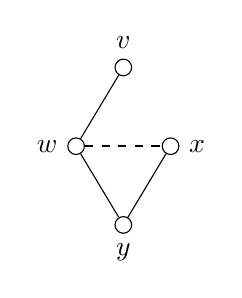
\begin{tikzpicture}[x=.6cm, y=1cm]
	\vertex (v) at (1,2) [label=above:$v$] {};
	\vertex (w) at (0,1) [label=left:$w$] {};
	\vertex (x) at (2,1) [label=right:$x$] {};
	\vertex (y) at (1,0) [label=below:$y$] {};
	\draw (v)--(w)--(y)--(x);
	\draw[thick, dashed] (w) -- (x);
	\end{tikzpicture}\]
	
You can scale the picture:\\
\[\begin{tikzpicture}[scale=1.5]
	\vertex (v) at (1,2) [label=above:$v$] {};
	\vertex (w) at (0,1) [label=left:$w$] {};
	\vertex (x) at (2,1) [label=right:$x$] {};
	\vertex (y) at (1,0) [label=below:$y$] {};
	\draw (v)--(w)--(y)--(x);
	\draw[thick, dashed] (w) -- (x);
	\end{tikzpicture}\]


 You can label edges.\\
 
\[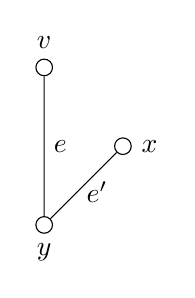
\begin{tikzpicture}
	\vertex (v) at (1, 2) [label=above:$v$]{};
	\vertex (x) at (2, 1) [label=right:$x$]{};
	\vertex (y) at (1, 0) [label=below:$y$]{};
	\draw (v) -- node[right]{$e$} (y) -- node[pos=.4,right]{$e'$} (x);
\end{tikzpicture}\]

For highly symmetric drawings, it is often easier to use polar coordinates. \\

\[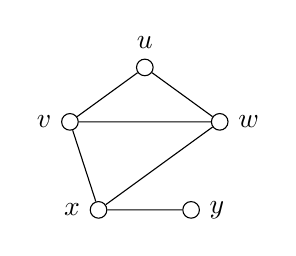
\begin{tikzpicture}
	\vertex (w) at (18:1) [label=right:$w$]{};
	\vertex (u) at (90:1) [label=above:$u$]{};
	\vertex (v) at (162:1) [label=left:$v$]{};
	\vertex (x) at (234:1) [label=left:$x$]{};
	\vertex (y) at (306:1) [label=right:$y$]{};
	\draw (y)--(x)--(w)--(u)--(v)--(x) (v)--(w);
\end{tikzpicture}\]

Leave off the labels if you want.\\
\[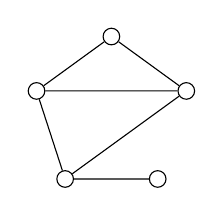
\begin{tikzpicture}
	\vertex (w) at (18:1) {};
	\vertex (u) at (90:1) {};
	\vertex (v) at (162:1) {};
	\vertex (x) at (234:1) {};
	\vertex (y) at (306:1) {};
	\draw (y)--(x)--(w)--(u)--(v)--(x) (v)--(w);
	\end{tikzpicture}\]

You can make vertices different colors.
	
\[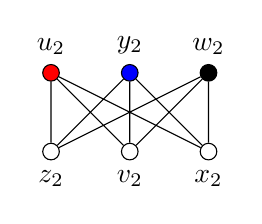
\begin{tikzpicture}
	\vertex[fill=red] (u2) at (0,1) [label=above:$u_{2}$] {};
	\vertex[fill=blue] (y2) at (1,1) [label=above:$y_{2}$] {};
	\vertex[fill] (w2) at (2,1) [label=above:$w_{2}$] {};
	\vertex (z2) at (0,0) [label=below:$z_{2}$] {};
	\vertex (v2) at (1,0) [label=below:$v_{2}$] {};
	\vertex (x2) at (2,0) [label=below:$x_{2}$] {};
	\draw (u2) -- (z2) -- (y2) -- (v2) -- (w2) -- (x2) -- (u2)-- (v2) -- (y2) -- (x2)(w2)--(z2);
	
	\end{tikzpicture}\]
 If you are willing to adjust the names of your vertices, you can use a ``for each" command to take advantage of symmetry.
 
 \[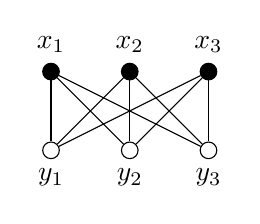
\begin{tikzpicture}
 	\foreach \i in {1,2,3}{
	\vertex[fill] (x\i) at (\i,1) [label=above:$x_{\i}$] {};
	\vertex (y\i) at (\i,0) [label=below:$y_{\i}$] {};
	}
	\foreach \i in {1,2,3}{
		\foreach \j in {1,2,3}{
		\draw (x\i) -- (y\j);
		}
	}
	\end{tikzpicture}\]


\end{document}
